\documentclass[addpoints,spanish, 12pt,a4paper]{exam}
%\documentclass[answers, spanish, 12pt,a4paper]{exam}
%\printanswers
\pointpoints{punto}{puntos}
\hpword{Puntos:}
\vpword{Puntos:}
\htword{Total}
\vtword{Total}
\hsword{Resultado:}
\hqword{Ejercicio:}
\vqword{Ejercicio:}

\usepackage[utf8]{inputenc}
\usepackage[spanish]{babel}
\usepackage{eurosym}
%\usepackage[spanish,es-lcroman, es-tabla, es-noshorthands]{babel}


\usepackage[margin=1in]{geometry}
\usepackage{amsmath,amssymb}
\usepackage{multicol}
\usepackage{yhmath}

\pointsinrightmargin % Para poner las puntuaciones a la derecha. Se puede cambiar. Si se comenta, sale a la izquierda.
\extrawidth{-2.4cm} %Un poquito más de margen por si ponemos textos largos.
\marginpointname{ \emph{\points}}

\usepackage{graphicx}
\graphicspath{{../img/}} 

\newcommand{\class}{1º Bachillerato CCSS}
\newcommand{\examdate}{\today}
\newcommand{\examnum}{Examen de números reales}
\newcommand{\tipo}{A}


\newcommand{\timelimit}{80 minutos}

\renewcommand{\solutiontitle}{\noindent\textbf{Solución:}\enspace}


\pagestyle{head}
\firstpageheader{
\includegraphics[width=0.2\columnwidth]{header_left}}{\textbf{Departamento de Matemáticas\linebreak \class}\linebreak \examnum}{
\includegraphics[width=0.1\columnwidth]{header_right}}
\runningheader{\class}{\examnum}{Página \thepage\ of \numpages}
\runningheadrule


\begin{document}

\noindent
\begin{tabular*}{\textwidth}{l @{\extracolsep{\fill}} r @{\extracolsep{6pt}} }
\textbf{Nombre:} \makebox[3.5in]{\hrulefill} & \textbf{Fecha:}\makebox[1in]{\hrulefill} \\
 & \\
\textbf{Tiempo: \timelimit} & Tipo: \tipo 
\end{tabular*}
\rule[2ex]{\textwidth}{2pt}
Esta prueba tiene \numquestions\ ejercicios. La puntuación máxima es de \numpoints. 
La nota final de la prueba será la parte proporcional de la puntuación obtenida sobre la puntuación máxima. 

\begin{center}


\addpoints
 %\gradetable[h][questions]
	\pointtable[h][questions]
\end{center}

\noindent
\rule[2ex]{\textwidth}{2pt}

\begin{questions}

\question[2] Indica a cuáles de los conjuntos
$\mathbb{N}$, $\mathbb{Z}$, $\mathbb{Q}$, $\mathbb{R}$ pertenecen cada uno de los siguientes números:
\begin{center}
\begin{tabular}{|c |c |c |c |c|}\hline
&$\mathbb{N}$& $\mathbb{Z}$& $\mathbb{Q}$&$\mathbb{R}$\\ 
\hline
$5$&&&&\\
\hline
$-7$&&&&\\
\hline
$0,23$&&&&\\
\hline
$\sqrt{\frac{18}{2}}$&&&&\\
\hline
$-\sqrt{3}$&&&&\\
\hline
$\sqrt[3]{-5}$&&&&\\
\hline
$4,\wideparen{7}$&&&&\\
\hline
$\frac{-\pi}{2}$&&&&\\
\hline
$-\sqrt{25}$&&&&\\
\hline
$\sqrt{-4}$&&&&\\
\hline
\end{tabular}

\end{center}

\begin{solution}
\begin{tabular}{|c |c |c |c |c|}\hline
&$\mathbb{N}$& $\mathbb{Z}$& $\mathbb{Q}$&$\mathbb{R}$\\ 
\hline
$5$&X&X&X&X\\
\hline
$-7$&&X&X&X\\
\hline
$0,23$&&&X&X\\
\hline
$\sqrt{\frac{18}{2}}$&X&X&X&X\\
\hline
$-\sqrt{3}$&&&&X\\
\hline
$\sqrt[3]{-5}$&&&&X\\
\hline
$4,\wideparen{7}$&&&X&X\\
\hline
$\frac{-\pi}{2}$&&&&X\\
\hline
$-\sqrt{25}$&&X&X&X\\
\hline
$\sqrt{-4}$&&&&\\
\hline
\end{tabular}
\end{solution}

\addpoints

\question Calcula:
%\noaddpoints % to omit double points count

\begin{parts}
\part[1] $\dfrac{1}{{1 - \sqrt {2} }} - \dfrac{{3 + 3\sqrt {2} }}{{\sqrt {2} \, - 4}}$ 
\begin{solution}
$\frac{\sqrt{2}}{14} + \frac{2}{7} $ 
\end{solution}
\part[1] $\dfrac{{\sqrt[5]{2\sqrt[4]{8}}  \cdot\sqrt {4\sqrt[3]{2}} }}{{\sqrt[12]{32} }}$
\begin{solution}
$2 \sqrt[10]{2} $
\end{solution}
\end{parts}

\question[1] Calcula un número que restado con el doble de su raíz cuadrada nos de 15.
\addpoints % to omit double points count
\begin{solution}
 	$- 2 \sqrt{x} + x - 15 = 0\to \left\{25\right\}$ 
\end{solution}

        \question Discute el tipo de sistema y resuelve si es posible:

        \begin{parts} \part[1]  $$ \left\{\begin{matrix}2x - y + z = 6\\ 2x + 2y - 4z = 2\\ x - 2y + 3z = 0\\ \end{matrix}\right. $$  \begin{solution}  $ \left[\begin{matrix}-1 & 2 & 1 & 6\\0 & 6 & -2 & 14\\0 & 0 & 0 & -5\end{matrix}\right] \rightarrow  \\ \left [ \right ] $  \end{solution} \part[1]  $$ \left\{\begin{matrix}x + 2y - 3z = 9\\ 4x - 2y = 12\\ 4x + 3y - 6z = 24\\ \end{matrix}\right. $$  \begin{solution}  $ \left[\begin{matrix}2 & 1 & -3 & 9\\0 & 5 & -3 & 21\\0 & 0 & 0 & 0\end{matrix}\right] \rightarrow  \\ \left \{ x : \dfrac{3 z}{5} + \dfrac{21}{5}, \quad y : \dfrac{6 z}{5} + \dfrac{12}{5}\right \} $  \end{solution}
        \end{parts}
        
\question[1] Sabiendo que log 3 = 0,477121, calcula
         
        \begin{parts} \part  $ \log(0.003) $  \begin{solution}  $ -2.52287875 $  \end{solution} \part  $ \log(\sqrt[ 4 ]{{0.03}^3}) $  \begin{solution}  $ -1.14215906 $  \end{solution} \part  $ \log(\sqrt[ 5 ]{0.81}) $  \begin{solution}  $ -0.0183029962 $  \end{solution} \part  $ \log(\frac{1}{81}) $  \begin{solution}  $ -1.90848502 $  \end{solution}
        \end{parts}
        

        
\question Resuelve:
 
        \begin{parts} \part[1]  $ \dfrac{{{x^3} - 5{x^2} + 2x + 8}}{x^2+1} < 0 $  \begin{solution}  $ \left(-\infty, -1\right) \cup \left(2, 4\right) $  \end{solution} 
        \end{parts}

\question Resuelve los siguientes sistemas de inecuaciones:
        \begin{parts} 
         \part[1]  $$ \left\{\begin{matrix}{( {x - 1} )^2} - {( {x + 3} )^2} \leq 0\\x - 3( {x - 1} ) \geq 3 \end{matrix}\right. $$  
         \begin{solution}  $ \left[-1, 0\right] $$  \end{solution}
         \part[1]  $$ \left\{\begin{matrix}x \geq 0 \\0 \leq y\\y \leq 3\\x - 2y \leq 10\\x + y \geq 10\\\end{matrix}\right. $$  \begin{solution}   \\ 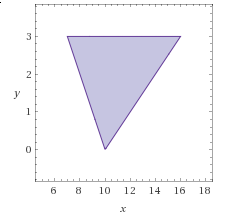
\includegraphics[width=1\columnwidth]{si5}   \end{solution}  
        \end{parts}




\addpoints

\end{questions}

\end{document}
\grid
